\documentclass[a4paper,12pt]{article} % Tipo de documento y tamaño de letra.
\usepackage[utf8]{inputenc} % Para que reconozca caracteres especiales como tildes.
\usepackage[spanish]{babel} % Para definir el idioma y el formato de fechas en español.
\usepackage{amsmath, amssymb} % Paquetes para símbolos y ecuaciones avanzadas (Para hacer una ecuación con un recuadro).
\usepackage{ragged2e} % Para justificar textos.
\usepackage{multicol} % Para crear columnas.
\usepackage{slashed} % Para generar números o variables canceladas (Una línea diagonal sobre el número o variable).
\usepackage{graphicx} % Paquete para poner graficas.
\usepackage{float} % Para poder dejar la imagen en un punto fijo del documento.
\usepackage{longtable} % Para tablas largas.
\usepackage{cancel} % Para hacer cancelaciones en medio de operaciones.
\usepackage{xcolor} % Para el color y esas cosas.
\usepackage{apacite} % Paquete para citas APA.
\usepackage{fancyhdr} % Para personalizar encabezados y pies de página.
\usepackage{geometry} % Para ajustar márgenes.
\usepackage{setspace} % Para ajustar el interlineado.
\usepackage{natbib} % Para manejar las citas y que no queden pegadas y feas :P.
\usepackage{hyperref} % Para que los enlaces funcionen con su URL.
\usepackage[version=4]{mhchem}  % Versión recomendada para mayor funcionalidad.
\usepackage{chemfig} %También para hacer estructuras químicas.
\usepackage{array} % Para mejor control de las columnas.
\usepackage{siunitx} % Para unidades físicas.


\pagestyle{fancy}
\fancyhf{} % Limpia encabezados y pies de página predeterminados
\fancyhead[L]{\textbf{ONDAS Y RELATIVIDAD.}} % Encabezado izquierdo
\fancyhead[R]{\textbf{FÍSICA ll}} % Encabezado derecho
\fancyfoot[C]{\thepage} % Número de página en el centro del pie

\geometry{headheight=12.96115pt, top=1in, bottom=1in, left=1in, right=1in}
\begin{document}


\begin{figure}[H] 
    \centering
    
\includegraphics[width=0.5\textwidth]{Unir.jpg} 
\end{figure}

\vspace{\baselineskip}

% Ajustamos manualmente todo ;)
\begin{center}
    \textbf{\Large } \\[0.3cm]
    \vspace{\baselineskip}
    \textbf{Liz Ángel Núñez Torres} \\[0.4cm]
    \textbf{Grado en Física} \\[0.4cm]
    \textbf{Universidad Internacional de La Rioja} \\[0.4cm]
    \textbf{07 de Marzo de 2025}
\end{center}


\newpage
\tableofcontents

\newpage

\begin{justify}
    Para el lector, queremos compartir la estructura visual del documento donde:
\end{justify}

\begin{itemize}
    \item Relegaremos los resultados \textbf{Definitivos} en un recuadro \textcolor{blue}{azul}.
    \item Relegaremos los resultados \textbf{Parciales} en un recuadro \textcolor{red}{rojo}.
\end{itemize}


\section{Ejercicio 1.}

\vspace{\baselineskip}

\begin{itemize}
    \item Una cuerda de 50.0 cm de longitud vibra sometida a una tensión de
    1.00 N. La Figura 1 muestra cinco imágenes estroboscópicas sucesivas de la cuerda. La lámpara
    produce 5000 destellos por minuto y las observaciones revelan que el desplazamiento máximo se
    dio en los destellos 1 y 5, sin otros máximos intermedios.
\end{itemize}

\begin{enumerate}
    \item Calcule la longitud de onda, el periodo y la frecuencia de las ondas que viajan por esta cuerda.
    \item ¿En qué modo normal (armónico) está vibrando la cuerda?.
    \item Calcule la rapidez de las ondas viajeras en la cuerda.
    \item ¿Con qué rapidez se está moviendo el punto P cuando la cuerda está en la posición 1 y la posición 3?.
\end{enumerate}

\vspace{\baselineskip}

\begin{figure}[H]
    \centering
    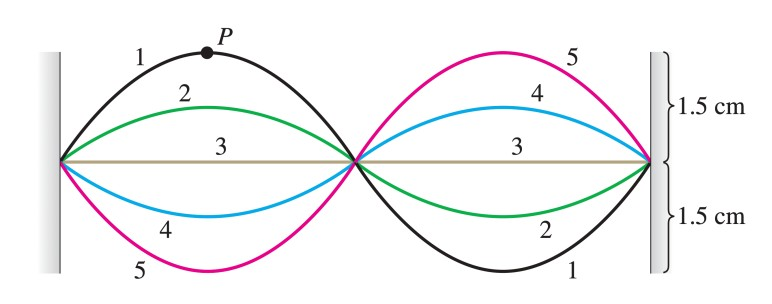
\includegraphics[width=0.5 \textwidth]{figura_1.jpg}
    \caption{Figura para la resolución del ejercicio 1.}
\end{figure}

\vspace{\baselineskip}

\subsection{Longitud de onda, Periodo, Frecuencia.}

\begin{justify}
Vamos a ordenar nuestros datos:
\end{justify}

\begin{justify}
    Primero, nos aseguramos en trabajar en el Sistema Internacional de Unidades \textbf{(SI)},

    \vspace{\baselineskip}

    \[ L = 50 \; \cancel{cm} \; \cdot \frac{1 \cancel{cm}}{100m} = 0.5m.   \]

    \[ f_s = 5000 \; d/ \cancel{m} \cdot \frac{1 \; \cancel{m}}{60s} = 83.3Hz. \]

    \[A = 1.5 \; \cancel{cm} \cdot \frac{1 \cancel{cm}}{100m} = 0.015m. \]

    \vspace{\baselineskip}

    \begin{justify}
        Denominaremos
        la \textbf{tensión} como \textbf{\((T_s)\)} y la \textbf{frecuencia de la lámpara estroboscópica}
        como \((f_s)\) para evitar confusiones de escritura con el \textbf{periodo} y la \textbf{frecuencia de la cuerda}.
    \end{justify}
\end{justify}

\begin{justify}
    Procedemos a organizar nuestros datos y a continuación, resolver las incognitas.
\end{justify}

\vspace{\baselineskip}

\begin{table}[h]
    \centering
    \renewcommand{\arraystretch}{1.5} % Espaciado vertical.
    \begin{tabular}{|>{\bfseries}l|r|} % Primera columna en negrita.
    \hline
    \multicolumn{1}{|c|}{\textbf{Variable}} & \multicolumn{1}{c|}{\textbf{Valor}} \\
    \hline
    Longitud \((L)\). & \( 0.5m.\)  \\
    \hline
    Tensión \((T_s)\). &\( 1.00N.\) \\
    \hline
    Frecuencia estroboscópica \((f_s)\). &  \(83.3Hz\). \\
    \hline 
    Amplitud \((A)\). & 0.015m. \\
    \hline
    Max.Desplazamiento. & 1 , 5. \\
    \hline
    \end{tabular}
    \caption{Datos sobre la cuerda vibrante.}
\end{table}

\vspace{\baselineskip}



\begin{justify}
    La \textbf{Longitud de onda} \((\lambda)\) por definición es la distancia que recorre una onda para completar un ciclo completo,
    en este caso, podemos hacer la relación matemática:
\end{justify}

\[ L = \lambda.\]

\[\textcolor{blue}{\boxed{\lambda = 0.5 \; m}}.\]

\vspace{\baselineskip}

\begin{justify}
    Aunque podemos usar la formula matemática \(\boxed{ \lambda = \frac{2L}{n}}\) donde \(n\) corresponde al número de modos, hemos prescindido de esta debido 
    a la intuitividad del punto trabajando con la definición y el análisis de la imagen.
\end{justify}

\vspace{\baselineskip}

\begin{justify}
    \textbf{Periodo (T)}. Como los máximos están en los destellos 1 y 5, podemos observar con la gráfica que entre estos existe \textbf{4 intervalos de tiempo} que cumplen
    \textbf{medio ciclo}, donde queda la relación:
\end{justify}

\[4 \; \Delta t = \frac{T}{2} \Rightarrow T = 2 \cdot 4 \; \Delta t \Rightarrow T = 8 \; \Delta t.\]

\vspace{\baselineskip}

\begin{justify}
    Aunque la imagen ya nos muestra a simple vista que el \textbf{destello 8} es el ciclo completo, hemos optado por usar una relación
    matemática para dar respuesta a este punto.
\end{justify}

\newpage 

\begin{justify}
    Un ciclo es la definición del \textbf{Periodo (T)}. Sin embargo, tendremos que saber cual es el valor de \(\Delta t\) para estimar el tiempo del ciclo completo, sabemos que
    los 5 destellos se producen en el tiempo \((f_s)\) de la lámpara, así que vamos a obtener el tiempo necesario para un solo destello, que es el valor \(\Delta t\).
    Una vez tengamos este tiempo, podremos saber el tiempo transcurrido en el destello 8, que es el ciclo completo. 
\end{justify}

\[\Delta t = \frac{1}{(f_s)} \Rightarrow \frac{1}{83.33} \Rightarrow \Delta t = 0.012s.\]

\vspace{\baselineskip}

\begin{justify}
    Por lo tanto, el \textbf{Periodo \((T)\)}:
\end{justify}

\[ T = 8 \cdot \Delta t \Rightarrow 8 \cdot 0.012s. \]

\[ \textcolor{blue}{\boxed{T = 0.096 s.}} \]

\vspace{\baselineskip} 

\begin{justify}
    \textbf{Frecuencia \((f)\)}. Para conocer el número de ciclos por segundo, necesitaremos el periodo \((T)\) dado que la frecuencia es el inverso de este.

\end{justify}

\[ f = \frac{1}{T} \Rightarrow f = \frac{1}{0.096s}.\]

\[ \textcolor{blue}{\boxed{f = 10.41 \; Hz.}}\]

\vspace{\baselineskip} 

\subsection{Modo armónico cuerda.}

\begin{justify}
    Usaremos una imagen para explicar este punto.
\end{justify}

\begin{figure}[H]
    \centering
    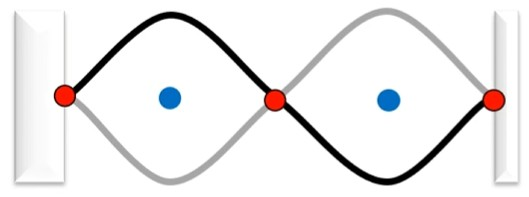
\includegraphics[width=0.5 \textwidth ]{figura_2.jpg}
    \caption{Onda estacionaria con tres nodos y dos antinodos.} 
\end{figure}

\begin{justify}
    En la imagen podemos observar los \textbf{nodos} \textcolor{red}{(Puntos de color rojo)} y los \textbf{antinodos} \textcolor{blue}{(Puntos azules)}.
    \begin{justify}
        El armónico es igual al número de antinodos, aunque también podemos afirmar que el número armónico es igual al número de nodos menos uno \((n_{armonico} = 1 - n ) \) donde 
        \(n\) es el número de nodos.
        \
    \end{justify}
\end{justify}

\vspace{\baselineskip}

\begin{center}
    \textcolor{blue}{\boxed{\text{Segundo modo normal } (n = 2)}}
\end{center}

\newpage

\subsection{Rapidez de la onda.}

\begin{justify}
    Para encontrar la rapidez de las ondas haremos el producto de la longitud de la onda \((\lambda)\) y la frecuencia \((f)\).
\end{justify}

\begin{justify}
    Esto debido a la definición de la velocidad, que es el cociente entre la distancia y el tiempo, que en nuestro caso el tiempo en recorrer la distancia es 
    el \textbf{Periodo}, y debido que el periodo es el inverso de la frecuencia tenemos:
\end{justify}

\[v = \frac{\lambda}{T} = \frac{\lambda}{\frac{1}{f}} \Rightarrow v = \lambda \cdot f.\]

\begin{justify}
    Por lo tanto:
\end{justify}

\[v = 0.5m \cdot 10.41 s^{-1}.\]

\vspace{\baselineskip}

\[\textcolor{blue}{\boxed{v = 5.20 \; m/s.}} \]

\vspace{\baselineskip}

\begin{justify}
    No usamos la formula \(v = \sqrt{\frac{T}{\mu}}\) porque desconocemos la densidad lineal \((\mu)\) y la masa \((m)\) para obtenerla, aunque si disponemos de la tensión.
\end{justify}

\vspace{\baselineskip}

\subsection{Rapidez en el punto P.}

\vspace{\baselineskip}

\begin{justify}
    \textbf{La posición 1} corresponde al antinodo en su máximo desplazamiento \textbf{(A)}, transversal a la dirección de la \textbf{onda sinusoidal} donde su desplazamiento es :
\end{justify}

\[x(t) = A \cdot \sin(\omega t).\]

\begin{justify}
    Donde el seno es máximo, \(\left(\sin (\frac{\pi}{2}) = 1\right)\). Así que al obtener la derivada de la función de onda, nos da la velocidad máxima en el punto \textbf{P}:  
\end{justify}

\[\frac{dx}{dt} = A \omega \cdot \cos\left(\frac{\pi}{2}\right) \Rightarrow A \omega  \cdot 0 = 0.\]

\begin{justify}
    Sin embargo, podemos argüir que la velocidad es cero porque al llegar la onda a su máxima amplitud, la cuerda se queda estatica en ese punto para regresar a su punto de equilibrio, por lo que la velocidad es cero.
\end{justify}

\[\textcolor{blue}{\boxed{v_{p1} = 0.}}\]

\newpage

\begin{justify}
    \textbf{La posición 3} corresponde al nodo donde se describe un movimiento armónico simple \textbf{(M.A.S)}, donde la derivada del coseno es \(\left(\cos(0) = 1\right)\) por lo tanto tenemos:
\end{justify}

\[ v_3 = A \omega \cdot \cos(0) \Rightarrow A \omega \cdot 1. \]

\begin{justify}
    \textbf{La frecuencia angular} \((\omega)\) es la velocidad angular de la onda, que se define como:

    \[ \omega = 2 \pi f \Rightarrow \omega = 2 \pi \cdot 10.41 s^{-1}. \]
\end{justify}

\begin{justify}
    Por lo tanto, la velocidad en el punto \textbf{P} es:
\end{justify}

\[ v_{p3} = A \cdot 2 \pi f \cdot 1 \Rightarrow 0.015m \cdot 2 \pi \cdot 10.41 s^{-1}. \]

\[ \textcolor{blue}{\boxed{v_{p3} = 0.981 \; m/s.}} \]

\vspace{\baselineskip}

\section{Ejercicio 2.}

\vspace{\baselineskip}

\begin{itemize}
    \item Una cuerda de guitarra de longitud \((L)\) se puntea, de modo que la onda
    total producida es la suma de la fundamental y el segundo armónico. 
    Es decir, la onda estacionaria está dada por:
\end{itemize}

\[y\left(t,x\right) = y_1(y,x) + y_2 (t,x).\]

Donde:

\[ y_1(t,x) = C \; \sin \left(\omega_1 t\right) \; \sin (k_1x). \]

\[ y_2(t,x) = C \; \sin \left(\omega_2 t\right) \; \sin (k_2x). \]

\begin{justify}
    Siendo \(\omega_1 = vk_1\) y \(\omega_2 = vk_2\):
\end{justify}

\begin{enumerate}
    \item ¿En qué valores de \(x\) están los nodos de \(y_1\)?.
    \item ¿Y los de \(y_2\)?.
    \item ¿La suma de las ondas estaionarias \(y_1\) e \(y_2\) produce una onda estacionaria?
    \item Explica.
\end{enumerate}

\newpage

\subsection*{1. Nodos de \( y_1 \)}

\vspace{\baselineskip}

\begin{justify}
    Los nodos de \( y_1(t, x) = C \sin(\omega_1 t) \sin(k_1 x) \) se encuentran donde la amplitud es siempre cero, es decir:
\end{justify}

\[ \sin(k_1 x) = 0 \implies k_1 x = n \pi \quad \text{con} \quad n \in \mathbb{Z}. \]

\begin{justify}
    Para el primer armónico, \( k_1 = \frac{\pi}{L} \), por lo que:
\end{justify}

\[ x = n L. \]

\begin{justify}
    Dado que \( x \in [0, L] \), los nodos están en:
\end{justify}

\[ \textcolor{blue}{\boxed{x = 0 \quad \text{y} \quad x = L.}}\]

\subsection{2. Nodos de \( y_2 \)}

\vspace{\baselineskip}

\begin{justify}
    Para \( y_2(t, x) = C \sin(\omega_2 t) \sin(k_2 x) \), los nodos cumplen:
\end{justify}

\[ \sin(k_2 x) = 0 \implies k_2 x = m \pi \quad \text{con} \quad m \in \mathbb{Z}. \]

\vspace{\baselineskip}

\begin{justify}
    Para el segundo armónico, \( k_2 = \frac{2\pi}{L} \), así que:
\end{justify}

\[ x = \frac{m L}{2}. \]

\begin{justify}
    En el intervalo \( [0, L] \), los nodos son:
\end{justify}


\[ \textcolor{blue}{\boxed{x = 0, \quad x = \frac{L}{2}, \quad \text{y} \quad x = L}}. \]

\vspace{\baselineskip}

\subsection{3. ¿Es \( y_1 + y_2 \) una onda estacionaria?}

\vspace{\baselineskip}

\begin{justify}
    La suma \( y(t, x) = y_1(t, x) + y_2(t, x) \) es una onda estacionaria debido que:
\end{justify}


\begin{itemize}
    \item Ambas componentes tienen frecuencias armónicas (\( \omega_2 = 2\omega_1 \)).
    \item Los nodos fijos en \( x = 0 \) y \( x = L \) se mantienen.
    \item La expresión puede escribirse como superposición de modos normales:
\end{itemize}

\[ y(t, x) = C \left( \sin(\omega_1 t) \sin\left(\frac{\pi x}{L}\right) + \sin(2\omega_1 t) \sin\left(\frac{2\pi x}{L}\right) \right).\]

\begin{justify}
    Podemos concluir finalmente que:
\end{justify}

\[ \textcolor{blue}{\boxed{\text{Sí, la suma } y_1 + y_2 \text{ produce una onda estacionaria.}}} \]



\section{Ejercicio 3.}

\vspace{\baselineskip}

\begin{itemize}
    \item Dos altavoces idénticos están situados en los puntos \(A\) y \(B\), separados
    \(2.00 m\). Los altavoces son alimentados por el mismo amplificador y producen ondas sonoras con
    una frecuencia de 784 Hz.

    La rapidez del sonido en aire es de 344 m/s. Un micrófono pequeño se
    aleja del punto \(B\) sobre una línea perpendicular a la línea que une a \(A\) y \(B\).
\end{itemize}

\begin{enumerate}
    \item ¿A qué distancias de B habrá interferencia destructiva?
    \item ¿Y constructiva? 
    \item  Si la frecuencia es lo bastante baja, no habrá posiciones sobre la línea BC en las que haya interferencia
        destructiva. ¿Qué tan baja deberá ser la frecuencia para que esto suceda?
\end{enumerate}

\begin{figure}[H]
    \centering
    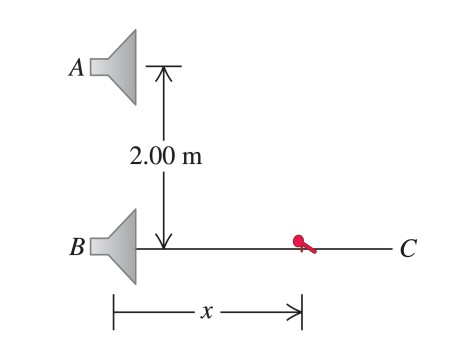
\includegraphics[width=0.5 \textwidth]{figura_3.jpg}
    \caption{Figura para la realización del ejercicio 3.}
\end{figure}

\vspace{\baselineskip}

\subsection{Distancia de B para interferencia destructiva.}


\begin{justify}
    Para que haya interferencia destructiva, la diferencia de camino \(\Delta r\) entre las ondas que llegan al micrófono
    desde los altavoces \(A\) y \(B\) debe ser igual a un número impar de longitudes de onda:
\end{justify}

\[ \Delta r = \left(n + \frac{1}{2}\right) \lambda \Rightarrow  n = (0.1.2,...).\]

\vspace{\baselineskip}

\begin{justify}
    La diferencia de camino \(\Delta r\) es la distancia entre los altavoces \(A\) y \(B\) a un punto \(P\) en la línea perpendicular \(AB\) a una distancia \(x\) de \(B\) menos la distancia entre \(B\) y \(P\).
\end{justify}

\begin{justify}
    Para el punto \(AP\) usamos el teorema de Pitágoras, de esta forma obtenemos que la diferencia de los caminos es.
\end{justify}

\[ \Delta r = AP - BP = \sqrt{x^2 + d^2} - x.\]

\begin{justify}
    Donde \(d\) es la distancia entre los altavoces \(A\) y \(B\), que es de \(2.00 m\). Esta expresión se iguala a la diferencia destructiva.
\end{justify}

\[ \sqrt{x^2 + d^2} -x = \left(n + \frac{1}{2}\right) \lambda.\]

\begin{justify}
    Elevamos al cuadrado ambos lados de la ecuación para eliminar la raíz cuadrada.
\end{justify}

\[ x^2 + d^2 = \left(x + \left(n + \frac{1}{2} \lambda\right)\right)^2.\]

\begin{justify}
    Expandiendo el lado derecho de la ecuación.
\end{justify}

\[ x^2 + d^2 = x^2 + 2x\left(n + \frac{1}{2}\right)\lambda + \left(n + \frac{1}{2}\right)^2 \lambda^2.\]

\[ d^2 = -\cancel{x^2} + \cancel{x^2} + 2x\left(n + \frac{1}{2}\right)\lambda + \left(n + \frac{1}{2}\right)^2 \lambda^2.\]

\[ 2x \left(n + \frac{1}{2}\right)\lambda = d^2 - \left(n + \frac{1}{2}\right)^2 \lambda^2. \]

\vspace{\baselineskip}

\[ \frac{\cancel{2}x \cancel{\left(n + \frac{1}{2}\right)\lambda}}{\cancel{2}\cancel{\left(n + \frac{1}{2}\right)\lambda}} = \frac{d^2 - \left(n + \frac{1}{2}\right)^2 \lambda^2 }{ 2\left(n + \frac{1}{2}\right)\lambda}.  \]

\vspace{\baselineskip}

\[ \textcolor{red}{\boxed{x = \frac{d^2 - \left(n + \frac{1}{2} \right)^2 \lambda^2}{2 \left(n + \frac{1}{2}\right) \lambda}.}}\]

\begin{justify}
    Obtenemos la longitud de onda \(\lambda\) recordando que la velocidad es \(344 \; m/s\) y la frecuencia \(784\) Hz.
\end{justify}

\[ \lambda = \frac{v}{f} \Rightarrow \frac{344 \; m/\cancel{s}}{784 \; \cancel{s^{-1}}}.\]

\vspace{\baselineskip}

\[ \lambda = 0.4387m. \]

\begin{justify}
    Sustituimos nuestros valores \(d\), \(\lambda\) y \(n\) en \((0,1,2)\) 
\end{justify}

\vspace{\baselineskip}

\begin{itemize}
    \item \(n = 0.\)
    
        \[x = \frac{2^2 - \left(0 + \frac{1}{2}\right)^2 0.4387^2 }{2\left(0 + \frac{1}{2}\right) 0.4387} = \frac{3.9951}{0.4387} = 9.10 \; m. \]
    
    \item \(n = 1.\)
    
    \[x = \frac{2^2 - \left(1 + \frac{1}{2}\right)^2 0.4387^2 }{2\left(1 + \frac{1}{2}\right) 0.4387} = \frac{3.76}{1.316} =  2.85  \; m. \]

    \item \(n = 2.\)
    
    \[x = \frac{2^2 - \left(2 + \frac{1}{2}\right)^2 0.4387^2 }{2\left(2 + \frac{1}{2}\right) 0.4387} = \frac{3.567}{2.1935} = 1.62 \; m. \]

\end{itemize}

\vspace{\baselineskip}

\begin{justify}
    Las distancias con referencia destructiva son \(\textcolor{blue}{\boxed{9.10 \; m, \; 2.85 \; m, \; 1.62 \; m}}\).
\end{justify}

\vspace{\baselineskip}


\subsection{Distancia B para interferencia constructiva}

\begin{justify}
    Para que haya interferencia constructiva la diferencia de caminos \( \Delta r\)  entre las ondas que llegan al micrófono desde los altavoces 
    \(A\) y \(B\) debe ser múltiplo entero de \(\lambda\). 
\end{justify}

\[ \Delta r = n \lambda \Rightarrow n = (0,1,2,...). \]

\begin{justify}
    Recordemos que la diferencia de caminos es la distancia entre los altavoces \(A\) y \(B\) a un punto P en la
    línea perpendicular \(AB\) a una distancia \(x\) de \(B\) menos la distancia entre \(B\) y \(P\). También que la distancia 
    \(AP\) la obtenemos con el teorema de Pitágoras.
\end{justify}

\[ \sqrt{x^2+d^2} -x = n \lambda. \]

\begin{justify}
    Procedemos a depejar \(x\) igual que el punto anterios.
\end{justify}

\[ x^2+d^2 = \left(x  +  n \;  \lambda \right)^2. \]

\[x^2 + d^2 = x^2 +2x \cdot n \lambda + n \lambda^2. \]

\[2x = \frac{-\cancel{x^2} + \cancel{x^2} + d^2 - n \lambda^2 }{n^2 \lambda}.\]

\[\textcolor{red}{\boxed{ x = \frac{d^2 -n^2 \lambda^2}{2 n \lambda }. }} \]

\vspace{\baselineskip}

\begin{justify}
    Si sustituimos por nuestros valores, donde conocemos la distancia \((d)\), la longitud de onda \((\lambda)\)
    y utilizamos los valores de \(n = \left(1,2,3\right)\) hemos omitido \( n=0 \) dado que este anula el resultado al obtener un \(\frac{0}{0}\).
\end{justify}

\begin{itemize}
    \item \(n = 1.\)
    
    \[ x = \frac{2^2 -1^2 \cdot 0,4387^2}{2 \cdot 1 \cdot 0,4387} = \frac{3.807}{0.8774} = 4.33 \; m. \]

    \item \(n = 2.\)
    
    \[x = \frac{2^2 -2^2 \cdot 0,4387^2}{2 \cdot 2 \cdot 0,4387 } = \frac{3.23}{1.75} = 1.845 \; m. \]

    \item \(n = 3.\)
    
    \[x = \frac{2^2 -3^2 \cdot 0,4387^2}{2 \cdot  3 \cdot 0,4387 } = \frac{2.268}{2.632} =  0.861 \; m. \]
\end{itemize}

\vspace{\baselineskip}

\begin{justify}
    Las distancias con referencias constructiva son:
\end{justify}

\[\textcolor{blue}{\boxed{4.33 \; m, 1.845 \; m, 0.861 \; m.}}\]

\newpage

\subsection{¿Qué tan baja debe ser la frecuencia para que no haya interferencia destructiva?}

\vspace{\baselineskip}

\begin{justify}
    Para que no exista interferencia de destructiva, los caminos de las ondas de los dos altavoces
    deben ser un múltiplo impar de media longitud de onda, por la definición de la interferencia destructiva que 
    dimos en el primer punto de este ejercicio, por esto tenemos que. 
\end{justify}

\[ d < \frac{\lambda}{2} \Rightarrow \lambda > 2d \Rightarrow \lambda = 4 \;m\]


\begin{justify}
    Como disponemos de la longitud de onda \((\lambda)\), vamos a calcular la frecuencia en esta, que sería la frecuencia 
    máxima para que \textbf{no} haya interferencia negativa.
\end{justify}

\[f = \frac{v}{\lambda} \Rightarrow \frac{344 \cancel{m}/s}{4 \; \cancel{m}}\]

\vspace{\baselineskip}

\[\textcolor{blue}{\boxed{ f = 86 \; \text{Hz}.}}\]


\section{Ejercicio 4.}

\begin{justify}
    Nicola Tesla, inventor del siglo XIX, propuso transmitir energía eléctrica
    por medio de ondas electromagnéticas sinusoidales. Suponga que se pretende transmitir energía
    eléctrica en un haz con área de sección transversal de \(100 \; m^2\).
\end{justify}

\begin{itemize}
    \item ¿Qué amplitudes de campo eléctrico y magnético se requieren para transmitir una cantidad de potencia equivalente a la que transportan
    las líneas de transmisión modernas (que conducen voltajes y corrientes del orden de \(500 kV\) y \(1000\) A)?
\end{itemize}

\vspace{\baselineskip}


\begin{justify}
    Tenemos los datos:
\end{justify}

\begin{table}[h]
    \centering
    \renewcommand{\arraystretch}{1.5} % Espaciado vertical.
    \begin{tabular}{|>{\bfseries}l|r|} % Primera columna en negrita.
    \hline
    \multicolumn{1}{|c|}{\textbf{Variable}} & \multicolumn{1}{c|}{\textbf{Valor}} \\
    \hline
    Área  \((A)\). & \( 100 \;m^2.\)  \\
    \hline
    Voltaje \((v)\). &\( 500 \; kV.\) \\
    \hline
    Corriente \((I)\). &  \(1000 \; A\). \\
    \hline
    \end{tabular}
    \caption{Datos sobre la energía y área de un haz.}
\end{table}

\vspace{\baselineskip}

\subsection{Amplitud del campo eléctrico.}

\vspace{\baselineskip}

\begin{justify}
    Definimos la potencia \((P)\) que se pretende transmitir dado que la necesitaremos para determinar la intensidad \((S)\) del haz.
\end{justify}

\[ P = v \cdot I. \Rightarrow 500.000 \; V \cdot 1000 \; A\]

\[ \textcolor{red}{\boxed{P = 5 \times 10^8 \; W}}\]

\vspace{\baselineskip}

\begin{justify}
    La intensidad \((S)\) determina la potencia en un área determinada.
\end{justify}

\[ S = \frac{P}{A} \Rightarrow \frac{5 \times 10^8 \; W }{100 \; m^2}. \]

\vspace{\baselineskip}

\[ \textcolor{red}{\boxed{S = 5 \times 10^6 \; W/m^2 .}} \]

\vspace{\baselineskip}

\begin{justify}
    Haremos entonces uso del \textbf{ vector Poynting} \((\vec{S})\) que en una \textbf{onda plana sinusoidal}, su magnitud es:
\end{justify}

\[ \vec{S} = \frac{1}{2} c \epsilon_0 E^2_0 . \]

\begin{justify}
    Donde:
\end{justify}

\begin{itemize}
    \item \( c = \) Velocidad de la luz \( \left(3 \times 10^8 \; m/s\right) .\)
    \item \( \epsilon_0 = \) Permitividad del vacío \( \left(8.85 \times 10^{-12} \; F/m \right).\)
    \item \( E_0 = \) Amplitud del campo eléctrico.
\end{itemize}

\begin{justify}
    Depejamos la amplitud del campo eléctrica \((E_0)\).
\end{justify}

\[ \frac{S}{\frac{1}{2}} = c \epsilon_0 E^2_0 \Rightarrow \frac{2S}{c \epsilon_0} = E^2_0 \Rightarrow E_0 = \sqrt{\frac{2S}{c \epsilon_0}}. \]

\vspace{\baselineskip}

\begin{justify}
    Sustituyendo por nuestro valores.
\end{justify}

\[ E_0 = \sqrt{\frac{2 \cdot 5 \times 10^6}{3 \times 10^8 \cdot 8.85 \times 10^{-12}}} \Rightarrow \sqrt{\frac{1.0 \times 10^7}{2.65 \times 10^{-3}}} \Rightarrow \sqrt{3.77 \times 10^9}. \]

\vspace{\baselineskip}

\[ \textcolor{blue}{\boxed{ E_0 = 6.1429 \times 10^4 \; V/m \Rightarrow 61.429 \; kV/m.}} \]

\vspace{\baselineskip}

\subsection{Amplitud del campo magnético.}

\begin{justify}
    Una vez obtenemos la amplitud del campo eléctrico, procedemos a obtener el campo magnético sabiendo que 
    una onda electromagnética se relaciona de la forma:
\end{justify}

\[ B_0 = \frac{E_0}{c} \Rightarrow \frac{6.1429 \times 10^4}{3 \times 10^8} \]

\vspace{\baselineskip}

\[ \textcolor{blue}{\boxed{B_0 = 2.047 \times 10^{-4} \; T.}} \]

\vspace{\baselineskip}

\section{Ejercicio 5.}

\vspace{\baselineskip}

\begin{justify}
    La nube de gas llamada Nebulosa del Cangrejo puede verse incluso con un telescopio pequeño; 
    es lo que queda de una supernova, es decir, una explosión de una estrella. 
    La explosión se vio en la Tierra el 4 de julio de 1054 D.C. Las serpentinas brillan con el color rojo
    característico de hidrógeno gaseoso caliente. En un laboratorio en la Tierra, el hidrógeno calentado
    produce luz roja con frecuencia de \( 4.568 \times 10^{14} \) Hz; la luz roja recibida de las extensiones de la
    nebulosa del Cangrejo que apuntan hacia la Tierra tienen una frecuencia de \( 4.586 \times 10^{14} \) Hz. 
\end{justify}

\begin{enumerate}
    \item Estima la rapidez con que estos bordes exteriores de la Nebulosa se están expandiendo. Supón que
    la rapidez del centro de la nebulosa relativa a la Tierra (lo que se denomina velocidad peculiar) es despreciable.

    \item Suponiendo que la rapidez de expansión ha sido constante desde la explosión de
    la supernova, estime el diámetro de la Nebulosa en metros y en años luz.

    \item El diámetro angular
    de la Nebulosa del Cangrejo vista desde la Tierra es de unos 5 minutos de arco (1 minuto de arco
    5 1 de grado). 60 Estime la distancia en años luz a la nebulosa, y estime el año en que tuvo lugar
    la explosión.
\end{enumerate}

\begin{justify}
    \textbf{Datos:}
\end{justify}

\begin{itemize}
    \item Velocidad de la luz  \( \Rightarrow c = 3 \times 10^8 m/s. \)
    \item Frecuencia de la luz en laboratorio \( \Rightarrow 4.568 \times 10^{14}. \)
    \item Frecuencia recibida desde la nebulosa del cangrejo \( \Rightarrow 4.586 \times 10^{14}. \)

\end{itemize}

\vspace{\baselineskip}

\subsection{Velocidad de expansión en los borde de exteriores de la nebulosa.}

\vspace{\baselineskip}

\begin{justify}
    Podemos argüir que la luz recibida por la nebulosa \textbf{se acerca}, dado que la \textbf{la frecuencia de la nebulosa es mayor} que la frecuencia 
    medida en el laboratorio. Esto indica un \textbf{corrimiento al azul} que denota acercamiento por parte de la luz emitida hacia el punto en el que nos situamos 
    que es la Tierra. 
\end{justify}

\begin{justify}
    A partir de este analisis, podemos optar por la fórmula del \textbf{efecto Doppler relativista} para una fuente de luz \textbf{que se acerca}.
\end{justify}

\[ \frac{v}{v_0} = \sqrt{\frac{1 + \beta}{1- \beta}} \]

\begin{justify}
    Donde \( (\beta)\) es el parámetro adimensional que representa la \textbf{velocidad relativa} entre la fuente que emite la luz y el observador.
    Procedemos a definir nuestras variables.
\end{justify}

\[ v = \text{Frecuencia recibida desde la nebulosa.} \]

\[ v_0 = \text{Frecuencia de la luz en el laboratorio.} \]

\[ \beta = \frac{v}{c}. \]

\vspace{\baselineskip}

\begin{justify}
    Depejamos \((\beta) \) para poder hallar la velocidad de expansión en los bordes de la nebulosa.
\end{justify}

\[ \frac{v}{v_0} = \sqrt{\frac{1 + \beta}{1- \beta}} \Rightarrow \left(\frac{v}{v_0}\right)^2 = \frac{1 + \beta}{1- \beta} \Rightarrow \left(\frac{v}{v_0}\right)^2 \left(1- \beta\right) = 1 + \beta \]

\vspace{\baselineskip}

\begin{justify}
    Sustituimos por nuestros datos:
\end{justify}

\[ \left(\frac{4.586}{4.568}\right)^2 \left(1 - \beta\right) = 1 + \beta \Rightarrow 1.0079 \cdot \left( 1 - \beta \right) = 1 + \beta. \]

\vspace{\baselineskip}

\[ 1.0079 - 1.0079\beta = 1 + \beta \Rightarrow 1.0079 - 1 = \beta + 1.0079\beta. \]

\[ 0.0079 = 2.079\beta \Rightarrow \beta = \frac{0.0079}{2.0079} \]

\[\textcolor{red}{\boxed{\beta = 0.00393}}\]

\vspace{\baselineskip}

\begin{justify}
    Una vez con el valor de \(\beta\), despejamos \(v\) para saber la velocidad de expansión.
\end{justify}

\[  \beta = \frac{v}{c} \Rightarrow v = \beta \cdot c .\]

\begin{justify}
    Hacemos la sustitución por los datos:
\end{justify}

\[ v = 0.000393 \cdot 3 \times 10^8 \]

\begin{justify}
    La velocidad de expansión en los bordes exteriores de la nebulosa del Cangrejo es.
\end{justify}

\[ \textcolor{blue}{\boxed{v = 1.179 \times 10^6 \; m/s}}\]

\vspace{\baselineskip}

\subsection{Diámetro de la nebulosa.}

\begin{justify}
    Suponiendo que la velocidad \((v)\) ha sido constante, vamos a calcular el tiempo desde que inicio la espansión.
    Para esto, basta con hacer una simple resta desde la actualidad hastael año de inicio , esto porque el año en que se registra en DC.
\end{justify}

\begin{itemize}
    \item Tiempo desde la expansión \( \Rightarrow 1054 - 2025 = \textcolor{red}{\boxed{971 \; \text{Años.}}} \)
    \item Velocidad de expansión \( \Rightarrow 1.179 \times 10^6 \; m/s \)
\end{itemize}

\begin{justify}
    Convertimos los años a segundos debido que la constante de la luz \((c)\) en el \textbf{(SI)} es metro sobre segundo.
\end{justify}

\[ t = 971 \; \cancel{\text{A}} \cdot \frac{365.25 \; \cancel{\text{D}}}{1 \; \cancel{\text{A}}} \cdot \frac{24 \; \cancel{\text{H}}}{1 \; \cancel{\text{D}}} \cdot \frac{3600 \; S}{1 \; \cancel{\text{H}}}. \]

\vspace{\baselineskip}

\[\textcolor{red}{\boxed{t = 3.064 \times 10^{10} \; s.}}\]

\begin{justify}
    Aunque puede parecer muy evidente, no vamos a escatimar en explicar los puntos.
\end{justify}

\begin{itemize}
    \item \( 365.25 \Rightarrow\) Porque estamos contando los años bisiestos.
    \item \( A \Rightarrow\) Años.
    \item \( D \Rightarrow\) Días.
    \item \( H \Rightarrow \) Horas.
\end{itemize}

\newpage

\begin{justify}
    Dado que cada partícula se aleja del centro a una misma velocidad, procederemos a calcular el radio como la distancia recorrida
    por una partícula desde el centro hasta el punto que está en la actualidad, porque el comportamiento es el de un \textbf{MRU} , esto lo plantearemos
    así porque \textbf{la velocidad es constante} en este supuesto.
\end{justify}

\[ d = r \Rightarrow r = v \cdot t \]

\[ r =  1.179 \times 10^6 \; m/\cancel{s} \cdot 3.064 \times 10^{10} \; \cancel{s}  \]

\[ \textcolor{red}{\boxed{ r = 3.612 \times 10^{16} \; m. }}\]

\begin{justify}
    Sabiendo que el diámetro \((D)\) es el doble del radio \((r)\).
\end{justify}


\[ D = 2r \Rightarrow 2 \cdot 3.612 \times 10^{16} \; m. \]

\[ \textcolor{blue}{ \boxed{D = 7.224 \times 10^{16} \; m.} }\]

\begin{justify}
    Debido que necesitamos la unidades en metros, vamos a obtener los metros que recorre la luz en un año.
    Sabemos que:
\end{justify}

\[ \text{1 Día} = 86.400 \; s \]

\begin{justify}
    Y como estamos contanto los años bisisestos.
\end{justify}

\[ 365.25 \ \cdot 86.400 \; = 3.15 \times 10 ^7 \; s. \]

\begin{justify}
    Obtenemos la distancia en metros respecto a \textbf{un año luz}.
\end{justify}

\[ 3 \times 10^8  m/\cancel{s} \cdot 3.15 \times 10^7 \; \cancel{s} \]

\[ \textcolor{red}{\boxed{ 9.46 \times 10^{15} \; m.}} \]

\begin{justify}
    El diámetro en años luz sería.
\end{justify}

\[ D = \frac{7.224 \times 10^{16} \; \cancel{m}.}{9.46 \times 10^{15} \; \cancel{m} } \]

\vspace{\baselineskip}

\[ \textcolor{blue}{\boxed{D = 7.63 \; \text{Años luz}}}\]

\vspace{\baselineskip}

\subsection{Distancia y año  de la explosión.}

\vspace{\baselineskip}

\begin{justify}
    Tenemos como datos.
\end{justify}

\begin{itemize}
    \item Diámetro lineal \((D) \Rightarrow 7.22 \times 10^{16} \; m \).
    \item Diámetro angular de la nebulosa \((\theta) \Rightarrow 5'. \) 
    \item Velocidad de la luz \((c) \Rightarrow 3 \times 10^8 m/s. \)
\end{itemize}

\begin{justify}
    Convertimos en radianes.
\end{justify}

\[ \frac{5}{60} \cdot \frac{\pi}{180}\]

\[ \textcolor{red}{\boxed{1.4544 \times 10^{-3} \; rad. }}\]

\vspace{\baselineskip}

\begin{justify}
    Relacionamos el diámetro lineal, diámetro angular y obtenemos la distancia de la tierra a la nebulosa.
\end{justify}

\[ \theta = \frac{D}{d} \Rightarrow d = \frac{D}{\theta}. \]

\begin{justify}
    Sustituimos por nuestros valores:
\end{justify}


\[ d = \frac{7.22 \times 10^{16} \; m}{1.4544 \times 10^{-3}} \]

\vspace{\baselineskip}

\[ \textcolor{red}{\boxed{ d = 4.96 \times 10^{19} \; m. }} \]

\vspace{\baselineskip}

\begin{justify}
    Obtenemos la distancia en años luz recordando la equivalencia del recorrido de la luz en metros obtenida en el punto anterior.
\end{justify}

\[ d = \frac{4.96 \times 10^{19} \; \cancel{m}.}{9.46 \times 10^{15} \; \cancel{m}} . \]

\vspace{\baselineskip}

\[ \textcolor{blue}{\boxed{d = 5.243 \; \text{Años luz.}}} \]

\begin{justify}
    Si usamos la distancia y la velocidad de expansión, podemos obtener el tiempo que tardo en obtener ese tamaño.
\end{justify}

\[  t = \frac{R}{v}. \]

\begin{justify}
    Sustituimos:
\end{justify}

\[ t = \frac{3.612 \times 10^{16} \; \cancel{m}}{1.179 \times 10^6 \; \cancel{m}/s}. \]

\vspace{\baselineskip}

\[ \textcolor{red}{\boxed{t = 3.063 \times 10^{10} \;s.}}  \]

\vspace{\baselineskip}

\begin{justify}
    Si pasamos segundo a años:
\end{justify}

\[ \frac{3.063 \times 10^{10} \cancel{s} }{365.25 \cdot 24 \cdot 3600 \; \cancel{s}} = 970 \; \text{Años} \]

\begin{justify}
    Si hacemos la resta obtenemos:
\end{justify}

\[ \textcolor{blue}{\boxed{2025 - 970 = 1055 \; d.C.}}\]

\begin{justify}
    Lo que nos daría un año de diferencia, cabe resaltar que para este supuesto \textbf{inter pretamos la velocidad como constante} cuando 
    normalmente esta debería disminuir paulatinamente, por esto podemos suponer que exista este desface de tiempo.
\end{justify}

\section{Ejercicio 6.}

\vspace{\baselineskip}

\begin{enumerate}
    \item Demuestra que la luz (o cualquier onda electromagnética) viaja a velocidad constante \(c\) y obtén una expresión para esa 
    velocidad en función de \(\epsilon_0\) y \(\mu_0\), partiendo de las ecuaciones de maxwell en su forma diferencial.
    
    \item Menciona las dos implicaciones que tenga este resultado.
\end{enumerate}

\vspace{\baselineskip}

\subsection{Demostración que una onda EM viaja a velocidad constante. }

\vspace{\baselineskip}

\begin{justify}
    Queremos demostrar que \(c = v\) cuando.
\end{justify}

\vspace{\baselineskip}

\[\textcolor{red}{\boxed{ c = \frac{1}{\sqrt{\epsilon_0 \mu_0}}.}} \]

\newpage

\begin{justify}
    Para demostralo, partiremos de las \textbf{ecuaciones de Maxwell} en el vacío.
\end{justify}

\begin{itemize}
    \item \( \nabla \cdot B = 0. \)
    \item \( \nabla \cdot E  = 0. \)
    \item \( \nabla \times E = - \frac{\partial B}{\partial t}. \)
    \item \( \nabla \times B = \mu_0 \epsilon_0 \frac{\partial E}{\partial t}. \)
\end{itemize}

\begin{justify}
    Tomaremos el rotacional de \(E\) (tercera ecuación) 
\end{justify}

\[ \nabla \times \left( \nabla \times E \right) = - \frac{\partial}{\partial t} \left( \nabla \times B \right) = - \mu_0 \epsilon_0 \frac{\partial^2 E}{\partial t^2}  \]

\begin{justify}
    Usando la identidad vectorial.
\end{justify}

\[ \nabla \times \left( \nabla \times E \right) = \nabla \left( \nabla \cdot E \right) - \nabla^2E \]

\begin{justify}
    Y dado que.
\end{justify}

\[ \nabla \cdot E = 0 \]

\begin{justify}
    Por la primera ecuación de Maxwell, por lo tanto.
\end{justify}

\[  - \nabla^2E = - \mu_0 \epsilon_0 \frac{\partial^2 E}{\partial t^2} \]

\[  \nabla^2E = \mu_0 \epsilon_0 \frac{\partial^2 E}{\partial t^2} \]

\vspace{\baselineskip}

\begin{justify}
    Recordemos que la ecuación de \textbf{onda clásica} es
\end{justify}

\[ \nabla^2 \psi = \frac{1}{v^2} \frac{\partial^2 \psi }{\partial t ^2} .\]

\vspace{\baselineskip}

\begin{justify}
    Donde \((\psi)\) es la función de onda, en nuestro caso \(E.\)
\end{justify}
\begin{justify}
    De las ecuaciones de Maxwell en el vacío, obtuvimos una expresión idéntica en forma a la ecuación general de onda, pero con un coeficiente distinto frente a la derivada temporal.
\end{justify}

\begin{justify}
    Para que ambas ecuaciones describan el mismo fenómeno, los coeficientes de las derivadas temporales deben ser equivalentes.
\end{justify}

\[ \mu_0 \epsilon_0 = \frac{1}{v^2}.\]

\begin{justify}
    Despejando \(v\).
\end{justify}

\[v^2 = \frac{1 }{ \mu_0 \epsilon_0}.\]

\vspace{\baselineskip}

\[ \textcolor{blue}{\boxed{v = \frac{1}{\sqrt{ \epsilon_0 \mu_0 }}}}. \]

\vspace{\baselineskip}


\subsection{Implicaciones.}

\begin{itemize}
    \item La velocidad de la luz es \textbf{constante} en \textbf{todos} los sistemas inerciales, esta invariancia
    parte de la \textbf{relatividad especial.}

    \item Confirma que la luz es un \textbf{onda electromagnética}, unificando la óptica física con el electromagnetismo.
\end{itemize}

\vspace{\baselineskip}


\section{Calificación/Observaciones.}

\begin{figure}[H]
    \centering
    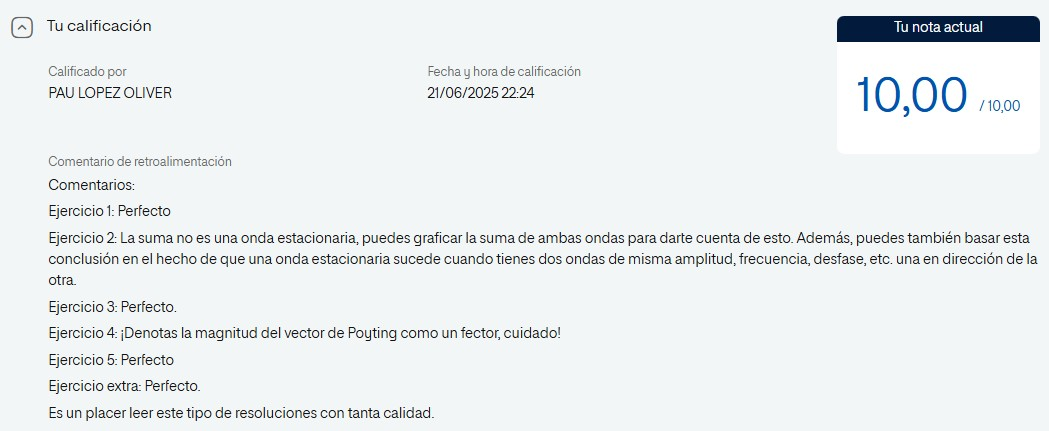
\includegraphics[width=1 \textwidth]{califiacion.jpg}
\end{figure}

\end{document}
